\title{Update to the identification guide to female Alaskan bumble bees and a summary of recent changes to the Alaskan bumble bee fauna}

\subtitle{\doi{10.----------}}

\author{by 
 Derek S.\ Sikes\footnote{University of Alaska Museum, Institute of Arctic Biology, University of Alaska Fairbanks, Fairbanks, Alaska, USA \email{dssikes@alaska.edu}} and
 Jessica J.\ Rykken\footnote{Denali National Park and Preserve, Alaska, USA \email{jessica\_rykken@nps.gov}}
 }

\maketitle

\end{multicols}

\vspace{-1cm}
\begin{center}
 \parbox[t][][s]{14cm}{\section{Summary}
 We summarize numerous recent changes to the taxonomy of the bumble bee fauna of Alaska since \citet{Pampell2010, Pampell2013}, \citet{KochStrange2012} and \citet{Pampelletal2012, Pampelletal2015}. Nine species are now referred to using different names and two new species were described.

 \begin{enumerate}
\item \citet{Williamsetal2014} resulted in the names \textit{Bombus bohemicus}, \textit{Bombus flavidus}, and \textit{Bombus cryptarum} replacing the previous names of \textit{Bombus ashtoni}, \textit{Bombus fernaldae}, and \textit{Bombus moderatus}, respectively. The former three names replace the latter three for all records in Alaska.

\item \citet{Williamsetal2015} elevated \textit{Bombus natvigi} and \textit{Bombus kirbiellus} from invalid as synonyms under \textit{Bombus hyperboreus} and \textit{Bombus balteatus}, respectively, to valid species status. All former records of \textit{B.\ hyperboreus} in Alaska are now \textit{B.\ natvigi}. All former records of \textit{B.\ balteatus} in Alaska are now \textit{B.\ kirbiellus}.

\item A new species, \textit{Bombus kluanensis}, was described by \citet{Williamsetal2016} from Yukon, Canada and Denali National Park and Preserve, Alaska.

\item Since 2017 we consider \textit{Bombus centralis} to be a doubtful member of the Alaskan fauna with all prior records of this species most likely being \textit{Bombus flavifrons}. 

\item \citet{Martinetetal2019} concluded \textit{Bombus sylvicola} is conspecific with \textit{Bombus lapponicus} and established it as a subspecies, thus all Alaskan \textit{Bombus sylvicola} are now \textit{Bombus lapponicus sylvicola}.

\item A new apparently rare species was described from the Alaskan Arctic: \textit{Bombus interacti} by \citet{Martinetetal2019}.

\item Since December 2019 we consider \textit{Bombus suckleyi} to be a doubtful member of the Alaskan fauna with all prior records of this species most likely being \textit{Bombus bohemicus}. 

\item \citet{Ghisbainetal2020} split \textit{Bombus bifarius} into two species and \textit{B.\ bifarius} does not occur in Alaska. All Alaskan \textit{B.\ bifarius} records should be considered \textit{Bombus vancouverensis}.

\item The Alaskan bumble bee fauna now has 22 confirmed species and 2 doubtful species for a possible total of 24 species.

\end{enumerate}
 }
\end{center}

\vspace{4mm}

\begin{multicols}{2}

\section{Introduction}

There has been a considerable increase in interest in pollinators, and specifically bumble bees, across North America. In part, this interest stems from concerns about observed bumble bee declines, especially in relation to effects from climate change, introduced pathogens, and habitat fragmentation \citep{Cameronetal2011, Kerretal2015, Soroyeetal2020}. In Alaska, there has also been interest in basic questions about species diversity, biology, and distribution \citet{KochStrange2012, Kochetal2012, Hattenetal2015, Pampelletal2015, Rykken2015, Rykken2017}. Since these published works there have been some taxonomic name changes, misidentifications discovered, new species described, and synonymies published which we summarize and comment on here to provide a handy reference for ongoing and future work on the Alaskan bee fauna. Numerous records in \href{https://www.gbif.org/}{GBIF.org} of Alaskan \textit{Bombus} exist under old taxonomic concepts or are misidentifications so such public data should be corrected or subsampled before use.

We have updated the color guide of \citet{Pampell2013} with these corrections and have made changes to the colors of some species figured in the guide to better match Alaskan populations. Note that identification of many species cannot be confirmed by color alone; there are other microscopic characters that may need examination (like malar length), so we strongly recommend this guide be used in conjunction with the \citet{Williamsetal2014} field guide. We also recommend the free PDF guide to bumble bees of the western states by \citet{Kochetal2012}. Color can vary within species (especially on tergites) and our updated guide shows primarily the most common conditions. Color is best observed on clean and dry specimens; it is very difficult to identify bumble bees with matted, dirty hairs. We have marked rarely collected species, those with fewer than 40 Alaskan specimens known to us, with an asterisk in the guide. A review of Alaskan \textit{Bombus} species with state conservation status assessments was recently completed by the Alaska Center for Conservation Science and can be found online (\url{https://accs.uaa.alaska.edu/wildlife/pollinator-diversity/}).

This guide is for female bumble bees. The guide can help for male identification, but males can show a higher degree of variability than females. Females have six visible abdominal (metasomal) segments called tergites, stingers, antennae with 10 flagellomeres, and their mandibles are wide apically and scoop-like. Males have seven visible tergites with the tip of their abdomen blunt and lacking a stinger, have antennae with 11 flagellomeres, and male mandibles are narrow and notably bearded.  

\section{Results}

\setcounter{subsection}{1}
\renewcommand\thesubsection{\arabic{section}}

\subsection{1) Replacement of the names \textit{Bombus ashtoni}, \textit{Bombus fernaldae}, and \textit{Bombus moderatus} by \textit{Bombus bohemicus}, \textit{Bombus flavidus}, and \textit{Bombus cryptarum}}

\citet{Williamsetal2014} resulted in the replacement of the names for three Alaskan species, \textit{Bombus ashtoni}, \textit{Bombus fernaldae}, and \textit{Bombus moderatus} by \textit{Bombus bohemicus}, \textit{Bombus flavidus}, and \textit{Bombus cryptarum}, respectively. The latter three names replace the former three for all records in Alaska. Details on the justifications for these changes can be found in \citet{Williamsetal2014} and the online catalog of \citet{Williams2020}, which cites \citet{Cameronetal2007} as justification for the first two. We have updated the names in the color guide accordingly (Figure \ref{color_guide}).

\end{multicols}
\begin{figure}[H]
\begin{center}
%\vspace{2mm}
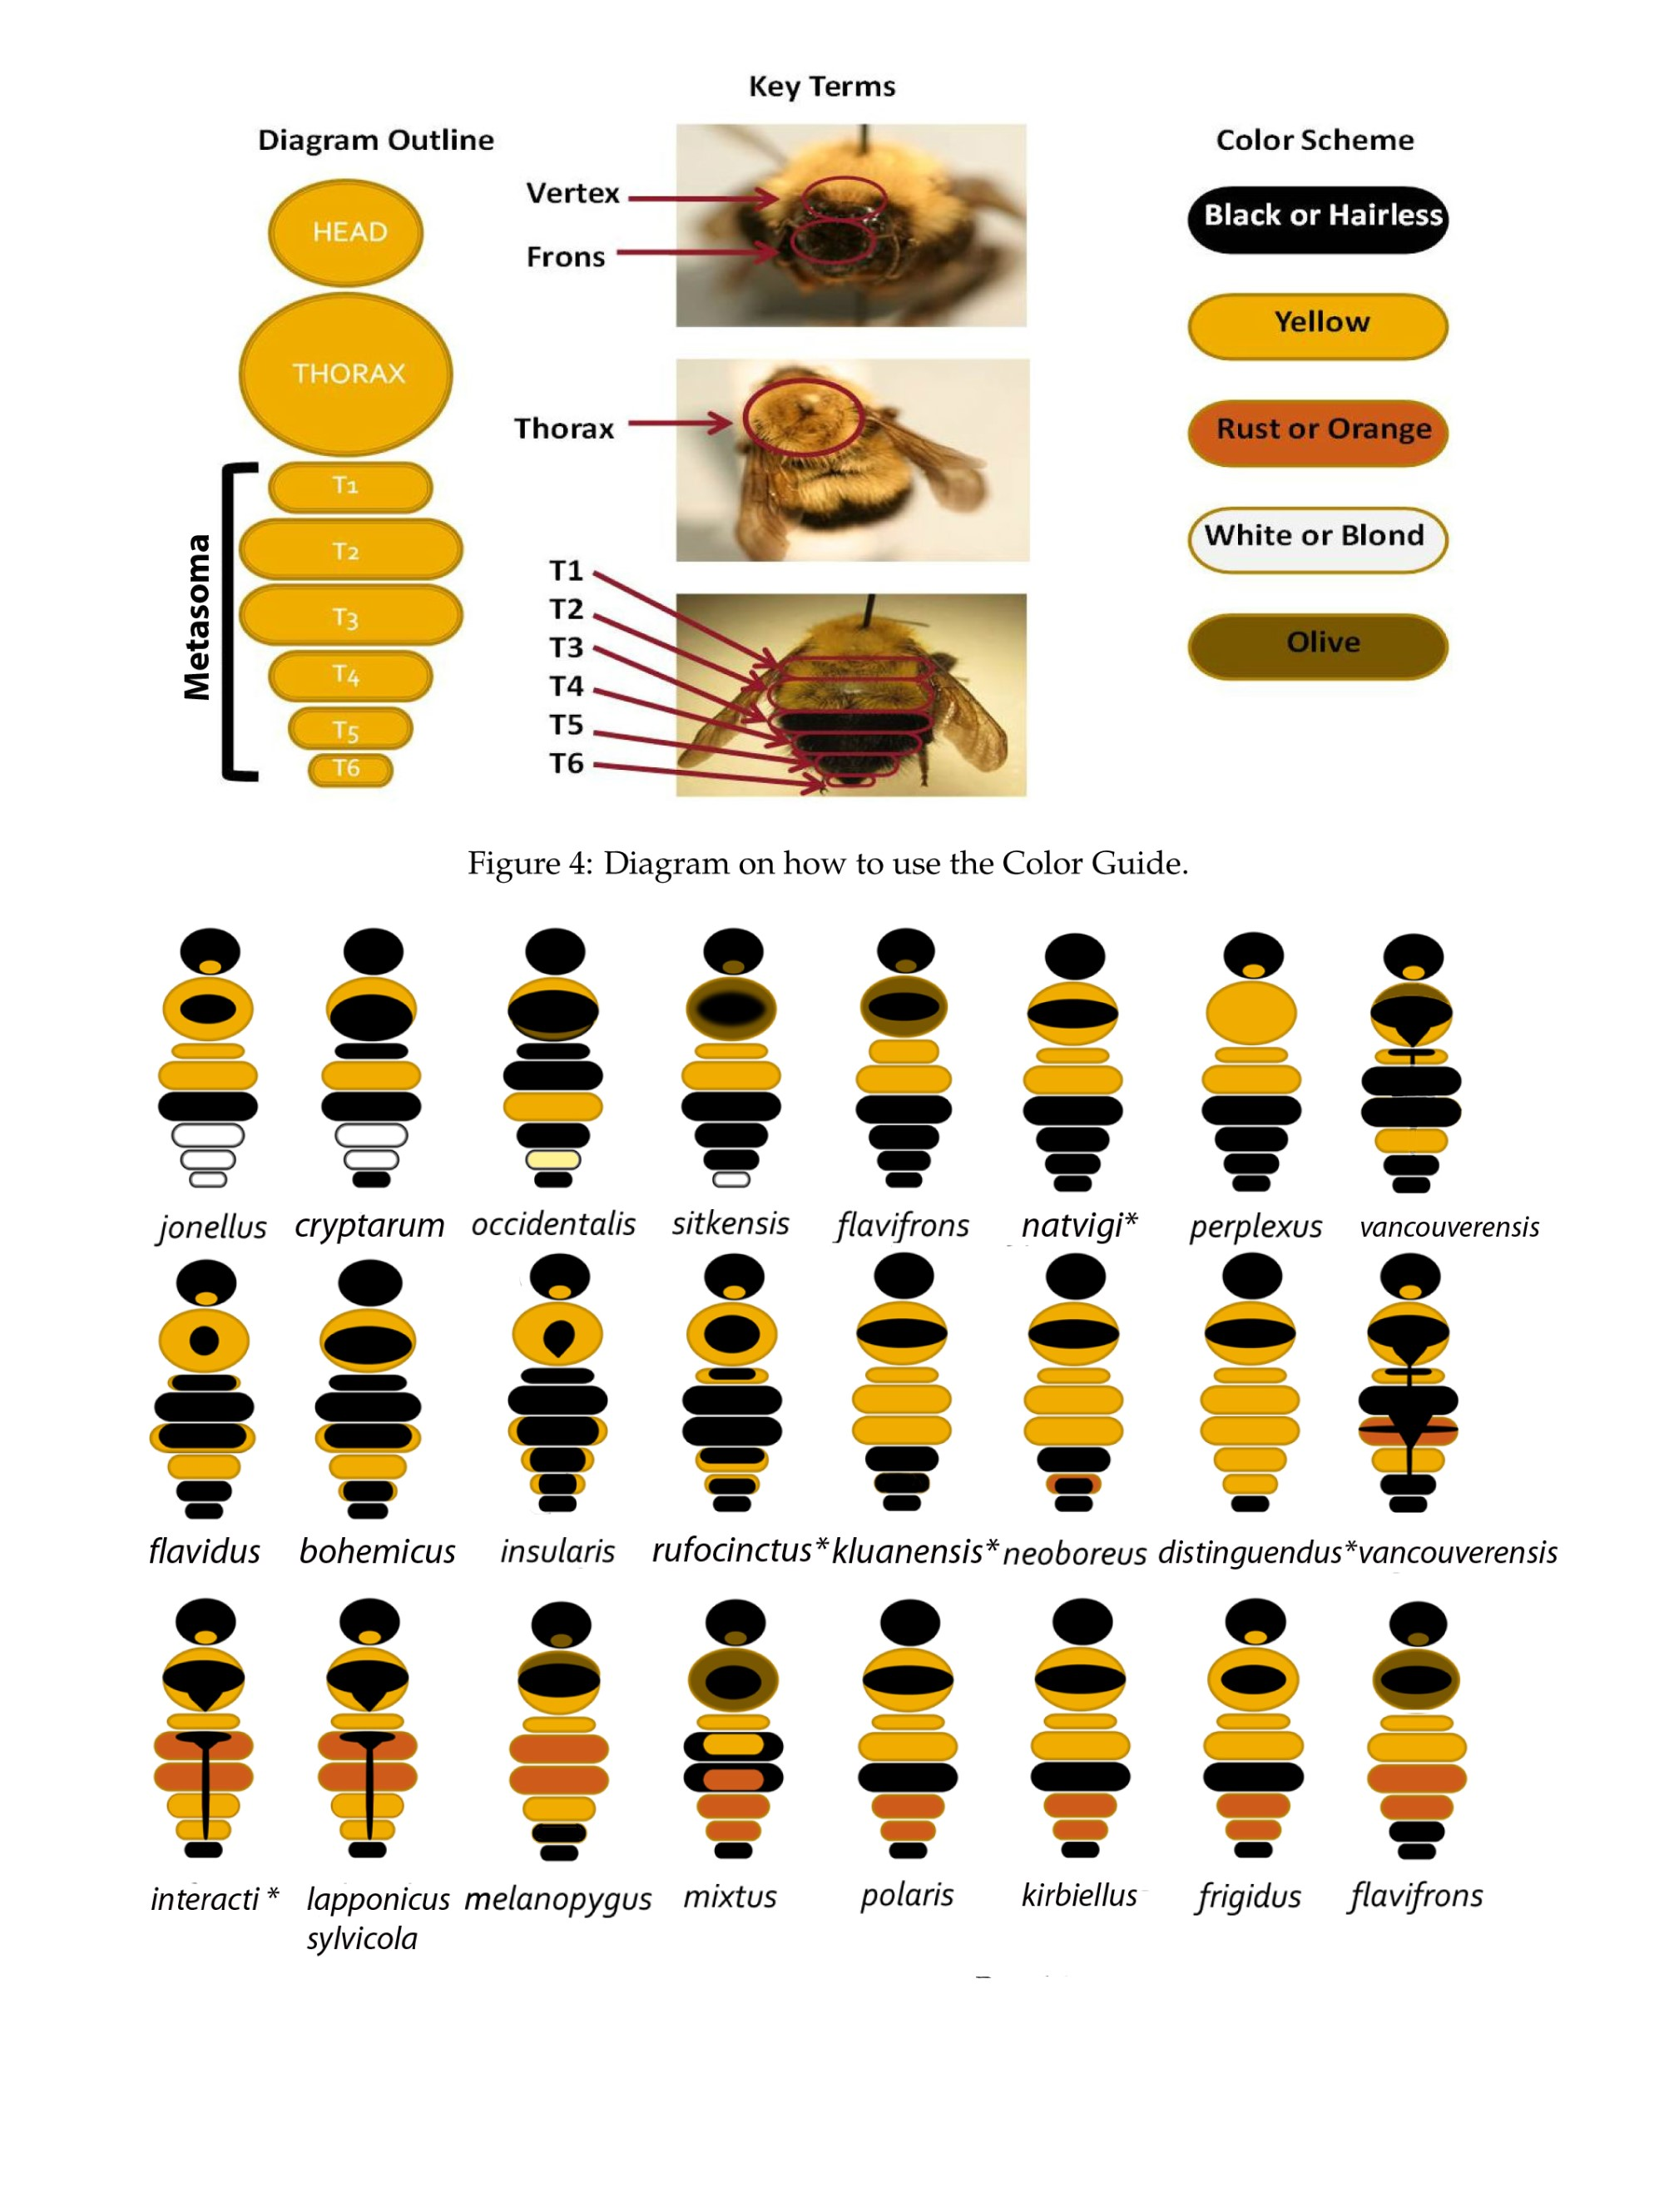
\includegraphics[width=\textwidth]{img/bumblebee_guide.jpg}
\caption{Color guide to common interior bumblebees of Alaska based on that of \citet{Pampell2010} with names and some colors updated. Rarely collected species, those with fewer than 40 Alaskan specimens known to us, are marked with an asterisk.}
\label{color_guide}
\end{center}
\end{figure} 
\begin{multicols}{2}

\bibliography{bumble_bee_update}

